\section{Convolution}

\begin{frame}{Introduction}
    \begin{enumerate}
        \item Using the convolution we can express the response of an LTI system to an arbitrary input in terms of the system's response to the unit impulse.
        \item An LTI system is completely characterized by its response to a single signal, namely, its response to the unit impulse.
        \item In discrete time, we have the convolution sum. In continuous time, we have the convolution integral.
        \item In this part of the course, we will learn to compute convolution sums and convolution integrals.
        \item In a latter section, under LTI system, we will obtain a thorough understanding of the concept of convolution.
    \end{enumerate}
\end{frame}

\begin{frame}{Convolution Sum}
    The convolution of the sequence $x[n]$ and $h[n]$ is given by
    \begin{equation}\label{eq:convolution_sum}
        y[n] = \sum_{k=-\infty}^{\infty}x[k]h[n-k],
    \end{equation}
    which we represent symbolically as
    \begin{equation}\label{eq:convolution_symbol}
        y[n] = x[n]\ast h[n]
    \end{equation}
\end{frame}

\begin{frame}{Example}
    Computer $y[n] = x[n]\ast h[n]$ for $x[n]$ and $h[n]$ as shown in Figure \ref{fi:example01_discrete_conv_signals}.
    \begin{figure}
      \centering
      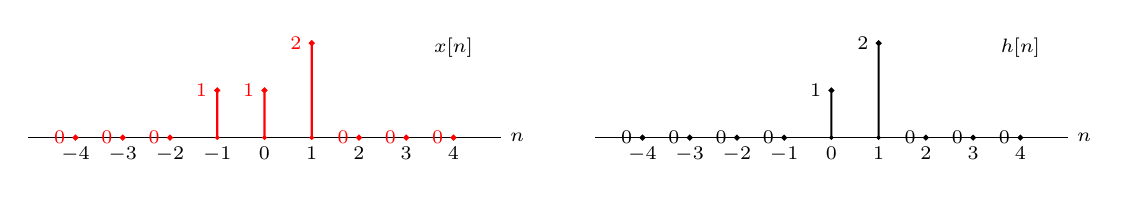
\begin{tikzpicture}[scale=0.6]

	\def\nmin{-4}
	\def\nmax{4}	
	
	\begin{scope}	
		\def\x{{0, 0, 0, 1, 1, 2, 0, 0, 0}}	

		\draw (\nmin-1, 0) -- (\nmax+1,0) node[anchor=west] {\scriptsize $n$};
		\foreach \n in {\nmin, ..., \nmax}
		{
			\node at (\n, 0) [anchor=north] {\scriptsize $\n$};
		}
		\node at (\nmax,1.5) [anchor=south] {\scriptsize $x[n]$};
		
		\foreach \n in {0,1, ...,8}
		{
			\pgfmathparse{\x[\n]}
			\edef\xn{\pgfmathresult}	
			\ifthenelse{\xn > 0}
			{
				\draw[red, thick, fill=red]  (\n + \nmin, 0) -- ++(0, \xn) circle (1pt) node[anchor=east] {\scriptsize $\xn$};
			}
			{
				\draw[red, fill=red] (\n+ \nmin,  0) circle (1pt);
			}
		}
	\end{scope}	
	
	\begin{scope}[xshift=12cm, yshift=0cm]	
		\def\h{{0, 0, 0, 0, 1, 2, 0, 0, 0}}	
		\draw (\nmin-1, 0) -- (\nmax+1,0) node[anchor=west] {\scriptsize $n$};
		\foreach \n in {\nmin, ..., \nmax}
		{
			\node at (\n, 0) [anchor=north] {\scriptsize $\n$};
		}
		\node at (\nmax,1.5) [anchor=south] {\scriptsize $h[n]$};
		
		\foreach \n in {0,1, ...,8}
		{
			\pgfmathparse{\h[\n]}
			\edef\hn{\pgfmathresult}	
			\ifthenelse{\hn > 0}
			{
				\draw[thick, fill=black]  (\n + \nmin, 0) -- ++(0, \hn) circle (1pt) node[anchor=east] {\scriptsize $\hn$};
			}
			{
				\draw[fill=black] (\n+ \nmin,  0) circle (1pt);
			}
		}
	\end{scope}		
	

\end{tikzpicture}


      \caption{Computing convolution}\label{fi:example01_discrete_conv_signals}
    \end{figure}        
\end{frame}

\begin{frame}<beamer>[plain,t]
    \begin{figure}
      \centering
      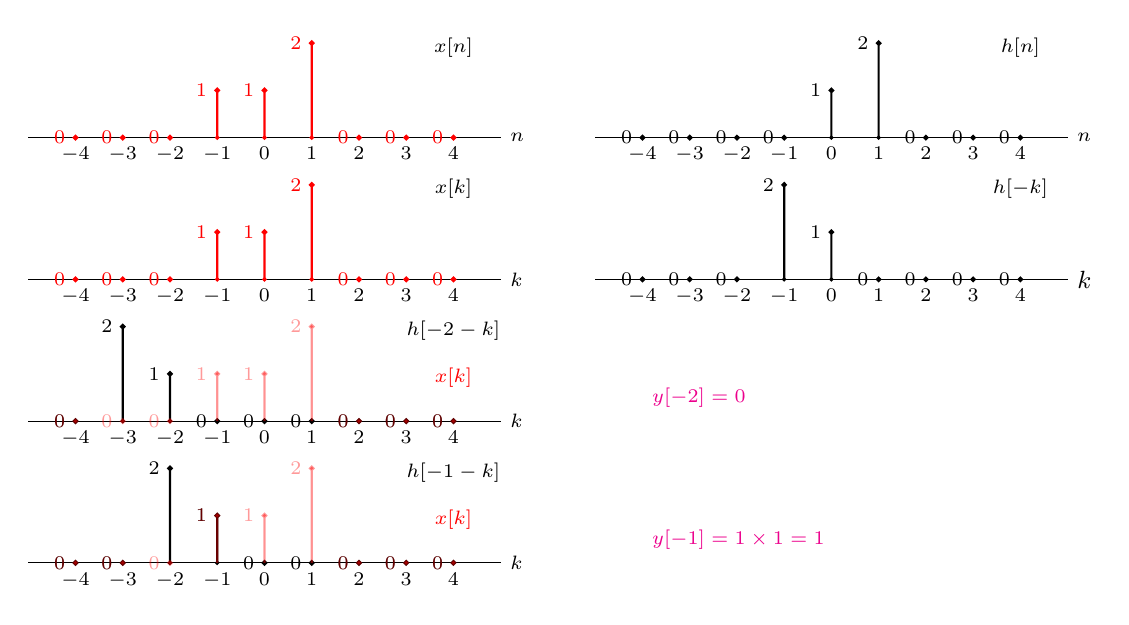
\begin{tikzpicture}[scale=0.6]

	\def\nmin{-4}
	\def\nmax{4}	
	
	\begin{scope}	
		\def\x{{0, 0, 0, 1, 1, 2, 0, 0, 0}}	

		\draw (\nmin-1, 0) -- (\nmax+1,0) node[anchor=west] {\scriptsize $n$};
		\foreach \n in {\nmin, ..., \nmax}
		{
			\node at (\n, 0) [anchor=north] {\scriptsize $\n$};
		}
		\node at (\nmax,1.5) [anchor=south] {\scriptsize $x[n]$};
		
		\foreach \n in {0,1, ...,8}
		{
			\pgfmathparse{\x[\n]}
			\edef\xn{\pgfmathresult}	
			\ifthenelse{\xn > 0}
			{
				\draw[red, thick, fill=red]  (\n + \nmin, 0) -- ++(0, \xn) circle (1pt) node[anchor=east] {\scriptsize $\xn$};
			}
			{
				\draw[red, fill=red] (\n+ \nmin,  0) circle (1pt);
			}
		}
	\end{scope}	
	
	\begin{scope}[xshift=12cm, yshift=0cm]	
		\def\h{{0, 0, 0, 0, 1, 2, 0, 0, 0}}	
		\draw (\nmin-1, 0) -- (\nmax+1,0) node[anchor=west] {\scriptsize $n$};
		\foreach \n in {\nmin, ..., \nmax}
		{
			\node at (\n, 0) [anchor=north] {\scriptsize $\n$};
		}
		\node at (\nmax,1.5) [anchor=south] {\scriptsize $h[n]$};
		
		\foreach \n in {0,1, ...,8}
		{
			\pgfmathparse{\h[\n]}
			\edef\hn{\pgfmathresult}	
			\ifthenelse{\hn > 0}
			{
				\draw[thick, fill=black]  (\n + \nmin, 0) -- ++(0, \hn) circle (1pt) node[anchor=east] {\scriptsize $\hn$};
			}
			{
				\draw[fill=black] (\n+ \nmin,  0) circle (1pt);
			}
		}
	\end{scope}		
	
	\begin{scope}[xshift=0cm, yshift=-3cm]		
		\def\x{{0, 0, 0, 1, 1, 2, 0, 0, 0}}	

		\draw (\nmin-1, 0) -- (\nmax+1,0) node[anchor=west] {\scriptsize $k$};
		\foreach \n in {\nmin, ..., \nmax}
		{
			\node at (\n, 0) [anchor=north] {\scriptsize $\n$};
		}
		\node at (\nmax,1.5) [anchor=south] {\scriptsize $x[k]$};
		
		\foreach \n in {0,1, ...,8}
		{
			\pgfmathparse{\x[\n]}
			\edef\xn{\pgfmathresult}	
			\ifthenelse{\xn > 0}
			{
				\draw[red, thick, fill=red]  (\n + \nmin, 0) -- ++(0, \xn) circle (1pt) node[anchor=east] {\scriptsize $\xn$};
			}
			{
				\draw[red, fill=red] (\n+ \nmin,  0) circle (1pt);
			}
		}
	\end{scope}	
	
	\begin{scope}[xshift=12cm, yshift=-3cm]	
		\def\h{{0, 0, 0, 2, 1, 0, 0, 0, 0}}	
		\draw (\nmin-1, 0) -- (\nmax+1,0) node[anchor=west] {\small $k$};
		\foreach \n in {\nmin, ..., \nmax}
		{
			\node at (\n, 0) [anchor=north] {\scriptsize $\n$};
		}
		\node at (\nmax,1.5) [anchor=south] {\scriptsize $h[-k]$};
		
		\foreach \n in {0,1, ...,8}
		{
			\pgfmathparse{\h[\n]}
			\edef\hn{\pgfmathresult}	
			\ifthenelse{\hn > 0}
			{
				\draw[thick, fill=black]  (\n + \nmin, 0) -- ++(0, \hn) circle (1pt) node[anchor=east] {\scriptsize $\hn$};
			}
			{
				\draw[fill=black] (\n+ \nmin,  0) circle (1pt);
			}
		}
	\end{scope}		
	
	\begin{scope}[xshift=0cm, yshift=-6cm]	
		\def\h{{ 0, 2, 1, 0, 0, 0, 0, 0, 0}}		
		\draw (\nmin-1, 0) -- (\nmax+1,0) node[anchor=west] {\scriptsize $k$};
		\foreach \n in {\nmin, ..., \nmax}
		{
			\node at (\n, 0) [anchor=north] {\scriptsize $\n$};
		}
		\node at (\nmax,1.5) [anchor=south] {\scriptsize $h[-2-k]$};
		
		\foreach \n in {0,1, ...,8}
		{
			\pgfmathparse{\h[\n]}
			\edef\hn{\pgfmathresult}	
			\ifthenelse{\hn > 0}
			{
				\draw[thick, fill=black]  (\n + \nmin, 0) -- ++(0, \hn) circle (1pt) node[anchor=east] {\scriptsize $\hn$};
			}
			{
				\draw[fill=black] (\n+ \nmin,  0) circle (1pt);
			}
		}
	\end{scope}		
	
	\begin{scope}[xshift=0cm, yshift=-9cm]	
		\def\h{{ 0, 0, 2, 1, 0, 0, 0, 0, 0}}		
		\draw (\nmin-1, 0) -- (\nmax+1,0) node[anchor=west] {\scriptsize $k$};
		\foreach \n in {\nmin, ..., \nmax}
		{
			\node at (\n, 0) [anchor=north] {\scriptsize $\n$};
		}
		\node at (\nmax,1.5) [anchor=south] {\scriptsize $h[-1-k]$};
		
		\foreach \n in {0,1, ...,8}
		{
			\pgfmathparse{\h[\n]}
			\edef\hn{\pgfmathresult}	
			\ifthenelse{\hn > 0}
			{
				\draw[thick, fill=black]  (\n + \nmin, 0) -- ++(0, \hn) circle (1pt) node[anchor=east] {\scriptsize $\hn$};
			}
			{
				\draw[fill=black] (\n+ \nmin,  0) circle (1pt);
			}
		}
	\end{scope}	
	
    \pause
	
	\begin{scope}[xshift=0cm, yshift=-6cm]		
		\def\x{{0, 0, 0, 1, 1, 2, 0, 0, 0}}	


		\node at (\nmax,.5) [anchor=south, red] {\scriptsize $x[k]$};
		
		\foreach \n in {0,1, ...,8}
		{
			\pgfmathparse{\x[\n]}
			\edef\xn{\pgfmathresult}	
			\ifthenelse{\xn > 0}
			{
				\draw[red, thick, fill=red, opacity=.4]  (\n + \nmin, 0) -- ++(0, \xn) circle (1pt) node[anchor=east] {\scriptsize $\xn$};
			}
			{

			}
		}
	\end{scope}		
	
	
	\begin{scope}[xshift=0cm, yshift=-9cm]		
		\def\x{{0, 0, 0, 1, 1, 2, 0, 0, 0}}	


		\node at (\nmax,.5) [anchor=south, red] {\scriptsize $x[k]$};
		
		\foreach \n in {0,1, ...,8}
		{
			\pgfmathparse{\x[\n]}
			\edef\xn{\pgfmathresult}	
			\ifthenelse{\xn > 0}
			{
				\draw[red, thick, fill=red, opacity=.4]  (\n + \nmin, 0) -- ++(0, \xn) circle (1pt) node[anchor=east] {\scriptsize $\xn$};
			}
			{

			}
		}
	\end{scope}			
	
    \pause
	
	\begin{scope}[xshift=8cm, yshift=-6cm]		

		\node at (0,.5) [anchor=west, magenta] {\scriptsize $y[-2] = 0$};
		
	\end{scope}		
	
	
	\begin{scope}[xshift=8cm, yshift=-9cm]		
		\node at (0,.5) [anchor=west, magenta] {\scriptsize $y[-1] = 1\times 1 = 1 $};
	\end{scope}		
\end{tikzpicture}


      \caption{Computing convolution}\label{fi:example01_discrete_conv_01}
    \end{figure}
\end{frame}

\begin{frame}<beamer>[plain,t]
    \begin{figure}
      \centering
      
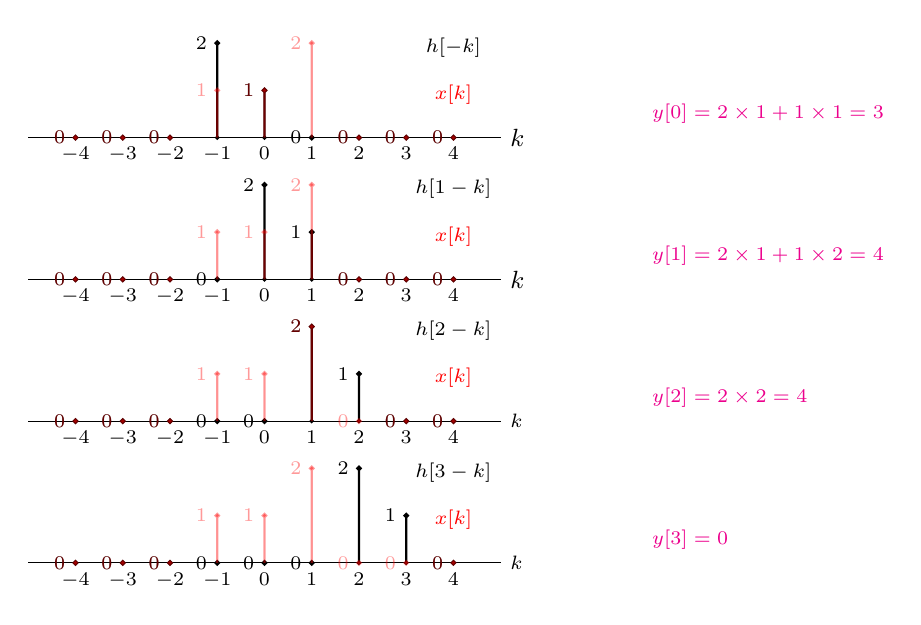
\begin{tikzpicture}[scale=0.6]
	\def\nmin{-4}
	\def\nmax{4}		
	\begin{scope}[xshift=0cm, yshift=0cm]	
		\def\h{{0,  0, 0, 2, 1, 0, 0, 0, 0}}		
		\draw (\nmin-1, 0) -- (\nmax+1,0) node[anchor=west] {\small $k$};
		\foreach \n in {\nmin, ..., \nmax}
		{
			\node at (\n, 0) [anchor=north] {\scriptsize $\n$};
		}
		\node at (\nmax,1.5) [anchor=south] {\scriptsize $h[-k]$};
		
		\foreach \n in {0,1, ...,8}
		{
			\pgfmathparse{\h[\n]}
			\edef\hn{\pgfmathresult}	
			\ifthenelse{\hn > 0}
			{
				\draw[thick, fill=black]  (\n + \nmin, 0) -- ++(0, \hn) circle (1pt) node[anchor=east] {\scriptsize $\hn$};
			}
			{
				\draw[fill=black] (\n+ \nmin,  0) circle (1pt);
			}
		}
	\end{scope}		


	\begin{scope}[xshift=0cm, yshift=-3cm]	
		\def\h{{0, 0,  0, 0, 2, 1, 0, 0, 0}}		
		\draw (\nmin-1, 0) -- (\nmax+1,0) node[anchor=west] {\small $k$};
		\foreach \n in {\nmin, ..., \nmax}
		{
			\node at (\n, 0) [anchor=north] {\scriptsize $\n$};
		}
		\node at (\nmax,1.5) [anchor=south] {\scriptsize $h[1-k]$};
		
		\foreach \n in {0,1, ...,8}
		{
			\pgfmathparse{\h[\n]}
			\edef\hn{\pgfmathresult}	
			\ifthenelse{\hn > 0}
			{
				\draw[thick, fill=black]  (\n + \nmin, 0) -- ++(0, \hn) circle (1pt) node[anchor=east] {\scriptsize $\hn$};
			}
			{
				\draw[fill=black] (\n+ \nmin,  0) circle (1pt);
			}
		}
	\end{scope}		


	\begin{scope}[xshift=0cm, yshift=-6cm]	
		\def\h{{0, 0, 0,  0, 0, 2, 1, 0, 0}}		
		\draw (\nmin-1, 0) -- (\nmax+1,0) node[anchor=west] {\scriptsize $k$};
		\foreach \n in {\nmin, ..., \nmax}
		{
			\node at (\n, 0) [anchor=north] {\scriptsize $\n$};
		}
		\node at (\nmax,1.5) [anchor=south] {\scriptsize $h[2-k]$};
		
		\foreach \n in {0,1, ...,8}
		{
			\pgfmathparse{\h[\n]}
			\edef\hn{\pgfmathresult}	
			\ifthenelse{\hn > 0}
			{
				\draw[thick, fill=black]  (\n + \nmin, 0) -- ++(0, \hn) circle (1pt) node[anchor=east] {\scriptsize $\hn$};
			}
			{
				\draw[fill=black] (\n+ \nmin,  0) circle (1pt);
			}
		}
	\end{scope}		
	
	\begin{scope}[xshift=0cm, yshift=-9cm]	
		\def\h{{0, 0, 0, 0,  0, 0, 2, 1, 0}}		
		\draw (\nmin-1, 0) -- (\nmax+1,0) node[anchor=west] {\scriptsize $k$};
		\foreach \n in {\nmin, ..., \nmax}
		{
			\node at (\n, 0) [anchor=north] {\scriptsize $\n$};
		}
		\node at (\nmax,1.5) [anchor=south] {\scriptsize $h[3-k]$};
		
		\foreach \n in {0,1, ...,8}
		{
			\pgfmathparse{\h[\n]}
			\edef\hn{\pgfmathresult}	
			\ifthenelse{\hn > 0}
			{
				\draw[thick, fill=black]  (\n + \nmin, 0) -- ++(0, \hn) circle (1pt) node[anchor=east] {\scriptsize $\hn$};
			}
			{
				\draw[fill=black] (\n+ \nmin,  0) circle (1pt);
			}
		}
	\end{scope}			

   \pause
	\begin{scope}[xshift=0cm, yshift=0cm]		
		\def\x{{0, 0, 0, 1, 1, 2, 0, 0, 0}}	


		\node at (\nmax,.5) [anchor=south, red] {\scriptsize $x[k]$};
		
		\foreach \n in {0,1, ...,8}
		{
			\pgfmathparse{\x[\n]}
			\edef\xn{\pgfmathresult}	
			\ifthenelse{\xn > 0}
			{
				\draw[red, thick, fill=red, opacity=.4]  (\n + \nmin, 0) -- ++(0, \xn) circle (1pt) node[anchor=east] {\scriptsize $\xn$};
			}
			{

			}
		}
	\end{scope}		
	

	\begin{scope}[xshift=0cm, yshift=-3cm]		
		\def\x{{0, 0, 0, 1, 1, 2, 0, 0, 0}}	


		\node at (\nmax,.5) [anchor=south, red] {\scriptsize $x[k]$};
		
		\foreach \n in {0,1, ...,8}
		{
			\pgfmathparse{\x[\n]}
			\edef\xn{\pgfmathresult}	
			\ifthenelse{\xn > 0}
			{
				\draw[red, thick, fill=red, opacity=.4]  (\n + \nmin, 0) -- ++(0, \xn) circle (1pt) node[anchor=east] {\scriptsize $\xn$};
			}
			{

			}
		}
	\end{scope}		
	

	\begin{scope}[xshift=0cm, yshift=-6cm]		
		\def\x{{0, 0, 0, 1, 1, 2, 0, 0, 0}}	


		\node at (\nmax,.5) [anchor=south, red] {\scriptsize $x[k]$};
		
		\foreach \n in {0,1, ...,8}
		{
			\pgfmathparse{\x[\n]}
			\edef\xn{\pgfmathresult}	
			\ifthenelse{\xn > 0}
			{
				\draw[red, thick, fill=red, opacity=.4]  (\n + \nmin, 0) -- ++(0, \xn) circle (1pt) node[anchor=east] {\scriptsize $\xn$};
			}
			{

			}
		}
	\end{scope}		
	

	\begin{scope}[xshift=0cm, yshift=-9cm]		
		\def\x{{0, 0, 0, 1, 1, 2, 0, 0, 0}}	


		\node at (\nmax,.5) [anchor=south, red] {\scriptsize $x[k]$};
		
		\foreach \n in {0,1, ...,8}
		{
			\pgfmathparse{\x[\n]}
			\edef\xn{\pgfmathresult}	
			\ifthenelse{\xn > 0}
			{
				\draw[red, thick, fill=red, opacity=.4]  (\n + \nmin, 0) -- ++(0, \xn) circle (1pt) node[anchor=east] {\scriptsize $\xn$};
			}
			{

			}
		}
	\end{scope}		
	
    \pause
	\begin{scope}[xshift=8cm, yshift=0cm]		

		\node at (0,.5) [anchor=west, magenta] {\scriptsize $y[0] = 2\times 1+ 1\times 1 = 3$};
		
	\end{scope}		
	
	
	\begin{scope}[xshift=8cm, yshift=-3cm]		
		\node at (0,.5) [anchor=west, magenta] {\scriptsize $y[1] = 2\times 1+ 1\times 2 = 4$};
	\end{scope}		    
	
	\begin{scope}[xshift=8cm, yshift=-6cm]		

		\node at (0,.5) [anchor=west, magenta] {\scriptsize $y[2] = 2\times 2 = 4$};
		
	\end{scope}		
	
	
	\begin{scope}[xshift=8cm, yshift=-9cm]		
		\node at (0,.5) [anchor=west, magenta] {\scriptsize $y[3] = 0$};
	\end{scope}		
	
\end{tikzpicture} 
      \caption{Computing convolution}\label{fi:example01_discrete_conv_02}
    \end{figure}
\end{frame}



\begin{frame}<beamer>[plain,t]
    \begin{figure}
      \centering
      
\begin{tikzpicture}[scale=0.6]
	\def\nmin{-4}
	\def\nmax{4}		
	\begin{scope}[xshift=0cm, yshift=0cm]	
		\def\y{{0,  0, 0, 1, 3, 4, 4, 0, 0}}		
		\draw (\nmin-1, 0) -- (\nmax+1,0) node[anchor=west] {\small $n$};
		\foreach \n in {\nmin, ..., \nmax}
		{
			\node at (\n, 0) [anchor=north] {\scriptsize $\n$};
		}
		\node at (\nmax,1.5) [anchor=south] {\scriptsize $y[n]$};
		
		\foreach \n in {0,1, ...,8}
		{
			\pgfmathparse{\y[\n]}
			\edef\hn{\pgfmathresult}	
			\ifthenelse{\hn > 0}
			{
				\draw[thick, fill=black]  (\n + \nmin, 0) -- ++(0, \hn) circle (1pt) node[anchor=east] {\scriptsize $\hn$};
			}
			{
				\draw[fill=black] (\n+ \nmin,  0) circle (1pt);
			}
		}
	\end{scope}		


	
	\begin{scope}[xshift=8cm, yshift=0cm]		
		\node at (0,.5) [anchor=west, magenta] {\scriptsize $y[n] = \begin{cases}0 & n \leq -2\\
		1 & n = -1\\ 3 & n = 0\\ 4 & n = 1\\ 4 & n = 2\\ 0 & n  \geq 3.
		\end{cases}$};
	\end{scope}		
	
\end{tikzpicture} 
      \caption{Computing convolution}\label{fi:example01_discrete_conv_03}
    \end{figure}
\end{frame}




\begin{frame}{Example}
    Consider and input $x[n]$ and a unit impulse response $h[n]$ given by 
    \begin{equation}
        \begin{split}
            x[n] &= \alpha^nu[n]'\\
            h[n] &= u[n],
        \end{split}
    \end{equation}
    which $0 < \alpha < 1$. Find $y[n]$ and sketch.
\end{frame}

\begin{frame}
    \begin{enumerate}
        \item
    \end{enumerate}
\end{frame}



